\documentclass[t]{beamer}

\usepackage{graphicx}
\usepackage{booktabs}
\usepackage{amsmath}
\usepackage{tikz}
\usepackage{tikz3d}
\usepackage{ifthen}
\usepackage[outline]{contour}
\usepackage{color}

% Grab the required TikZ libraries
\usetikzlibrary{ hexagon
               , calc
               , backgrounds
               , positioning
               , automata
               , shadows
               , fit
               , shapes
               }

%% Cache TikZ figures
%\usetikzlibrary{external}
%\tikzexternalize[prefix=tikzcache/]

% Use the UoM Beamer Theme
\usetheme[darktitle,cabin,framenumber,totalframenumber]{UniversityOfManchester}


\title{Improving the Interconnection Network of a Brain Simulator}
\subtitle{End-of-Year Presentation}
\author{Jonathan Heathcote}
\date{}

\begin{document}
	
	\maketitle
	
	\begin{frame}{(Artificial) Neural Networks}
		\center
		\only<1>{\input{|"python figures/ann-example.py 0"}}%
		\only<2>{\input{|"python figures/ann-example.py 1"}}%
		%Enable Me!
	\end{frame}
	
	\begin{frame}{Tree Topology}
		\center
		\begin{tikzpicture}[thick, node distance=1em,level distance=1.2cm]
	
	% Bodge/Hack to vertically center with mesh and torus figures.
	\draw [white] (-1.3cm,-3.85cm) rectangle ++(2cm,2cm);
	
	\begin{scope}[every node/.style={draw,rectangle,thick},             inner sep=0.1cm]
		\tikzstyle{level 1}=[sibling distance=2.4cm,every child/.style  ={},inner sep=0.1cm]
		\tikzstyle{level 2}=[sibling distance=1.2cm,every child/.style  ={},inner sep=0.1cm]
		\tikzstyle{level 3}=[sibling distance=0.6cm,every child/.style={},inner sep=0.1cm]
		
		\node {}
			child {node {}
				child {node {}
					child {node [fill,circle] {}}
					child {node [fill,circle] {}}
				}
				child {node {}
					child {node [fill,circle] {}}
					child {node [fill,circle] {}}
				}
			}
			child {node {}
				child {node {}
					child {node [fill,circle] {}}
					child {node [fill,circle] {}}
				}
				child {node {}
					child {node [fill,circle] {}}
					child {node [fill,circle] {}}
				}
			}
		;
	\end{scope}
	
\end{tikzpicture}


	\end{frame}
	
	\begin{frame}{Torus Topology}
		\center
		\begin{tikzpicture}[thick,inner sep=0.1cm,3d/perspective eye={0,10,20}]
	\def\width{5}
	\def\height{5}
	
	\def\tubewidth{1}
	\def\holesize{5}
	
	\pgfmathtruncatemacro{\widthh}{\width - 1}
	\pgfmathtruncatemacro{\heightt}{\height - 1}
	
	\clip (-0.7,-0.5) rectangle (\widthh+0.7,\heightt+0.7);
	
	\foreach \lx in {0,...,\widthh}{
		\foreach \ly in {0,...,\heightt}{
			\node [fill,circle]
			      (node X\lx Y\ly) at (\lx, \ly)
			      {};
		}
	}
	
	% Draw normal links
	\foreach \x in {0,...,\widthh}{
		\foreach \y in {0,...,\heightt}{
			\pgfmathtruncatemacro{\xx}{\x + 1}
			\pgfmathtruncatemacro{\yy}{\y + 1}
			\ifthenelse{\xx < \width}{
				\draw (node X\x Y\y.center) -- (node X\xx Y\y.center);
			}{
				%\draw (node X\x Y\y.center) -- (node X0Y\y.center);
			}
			\ifthenelse{\yy < \height}{
				\draw (node X\x Y\y.center) -- (node X\x Y\yy.center);
			}{
				%\draw (node X\x Y\y.center) -- (node X\x Y0.center);
			}
		}
	}
	
	% Draw Long Links
	\foreach \x in {0,...,\widthh}{
		\draw  (node X\x Y0.center)
		            .. controls +(0.7,-2.0)
		                    and +(0.7,2.0)
		            .. (node X\x Y\heightt.center);
	}
	\foreach \y in {0,...,\heightt}{
		\draw  (node X0Y\y.center)
		            .. controls +(-2.0,0.7)
		                    and +(2.0,0.7)
		            .. (node X\widthh Y\y.center);
	}
	
\end{tikzpicture}


	\end{frame}
	
	\begin{frame}{Wiring Constraints}
		\begin{itemize}
			\item \textbf{Cheap} Cables
			\item \textbf{Short} Cables
			\item \textbf{Easy} to Assemble (by a human)
		\end{itemize}
	\end{frame}
	
	\begin{frame}[c]{SpiNNaker in Cabinets}
		\hspace*{-0.1\textwidth}
		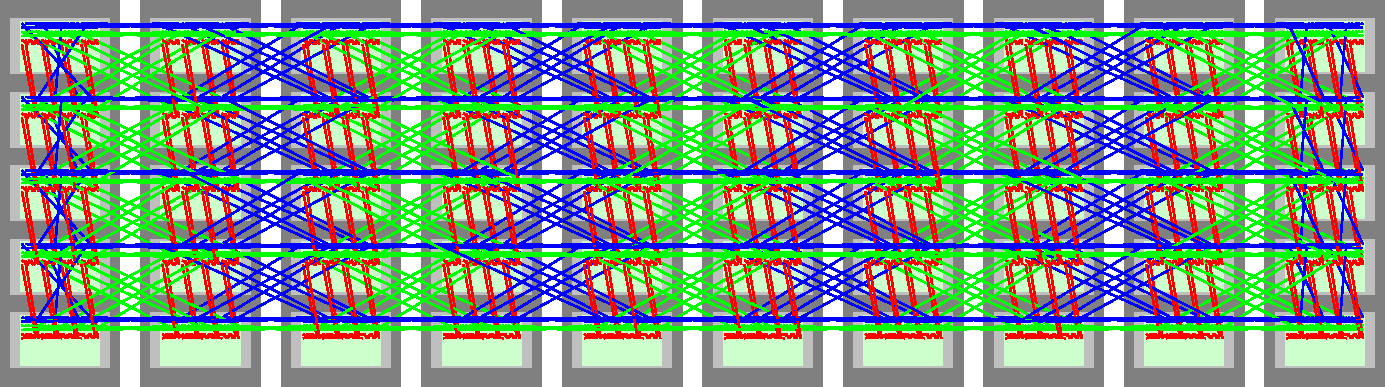
\includegraphics[width=1.2\textwidth]{figures/spinnaker106}
	\end{frame}
	
	\begin{frame}{Small-World Topology}
		% XXX: F'n beamer...
		\only<1>{\hspace{2cm}\begin{tikzpicture}[thick,inner sep=0.1cm,scale=0.8]
	\clip (-0.5,-0.5) rectangle (5.5,5.5);
	
	\node [fill,circle] (node 163015180) at (0,0) {};
	\node [fill,circle] (node 169393228) at (1,0) {};
	\node [fill,circle] (node 169393132) at (2,0) {};
	\node [fill,circle] (node 169393324) at (3,0) {};
	\node [fill,circle] (node 169393420) at (4,0) {};
	\node [fill,circle] (node 169393548) at (5,0) {};
	\node [fill,circle] (node 169393708) at (0,1) {};
	\node [fill,circle] (node 169393836) at (1,1) {};
	\node [fill,circle] (node 169393868) at (2,1) {};
	\node [fill,circle] (node 169393932) at (3,1) {};
	\node [fill,circle] (node 169393964) at (4,1) {};
	\node [fill,circle] (node 169394092) at (5,1) {};
	\node [fill,circle] (node 169521292) at (0,2) {};
	\node [fill,circle] (node 169521388) at (1,2) {};
	\node [fill,circle] (node 169521420) at (2,2) {};
	\node [fill,circle] (node 169521452) at (3,2) {};
	\node [fill,circle] (node 169521516) at (4,2) {};
	\node [fill,circle] (node 169527788) at (5,2) {};
	\node [fill,circle] (node 169543532) at (0,3) {};
	\node [fill,circle] (node 169544076) at (1,3) {};
	\node [fill,circle] (node 169544332) at (2,3) {};
	\node [fill,circle] (node 169544908) at (3,3) {};
	\node [fill,circle] (node 169545132) at (4,3) {};
	\node [fill,circle] (node 169574508) at (5,3) {};
	\node [fill,circle] (node 169575276) at (0,4) {};
	\node [fill,circle] (node 169576140) at (1,4) {};
	\node [fill,circle] (node 169601164) at (2,4) {};
	\node [fill,circle] (node 169599660) at (3,4) {};
	\node [fill,circle] (node 169646988) at (4,4) {};
	\node [fill,circle] (node 169647084) at (5,4) {};
	\node [fill,circle] (node 169647212) at (0,5) {};
	\node [fill,circle] (node 169647308) at (1,5) {};
	\node [fill,circle] (node 169647340) at (2,5) {};
	\node [fill,circle] (node 169647372) at (3,5) {};
	\node [fill,circle] (node 169647404) at (4,5) {};
	\node [fill,circle] (node 169647500) at (5,5) {};
	
	\draw (node 163015180) -- (node 169393228);
	\draw (node 163015180)
							         .. controls +(-1.000000,0.500000)
							                 and +(1.000000,0.500000)
							         .. (node 169393548);
	\draw (node 163015180)
							         .. controls +(0.500000,-1.000000)
							                 and +(0.500000,1.000000)
							         .. (node 169575276);
	\draw (node 163015180)
							         .. controls +(0.500000,-1.000000)
							                 and +(0.500000,1.000000)
							         .. (node 169647212);
	\draw (node 169393228) -- (node 169647500);
	\draw (node 169393228) -- (node 169393836);
	\draw (node 169393228)
							         .. controls +(0.500000,-1.000000)
							                 and +(0.500000,1.000000)
							         .. (node 169647308);
	\draw (node 169393132) -- (node 169393324);
	\draw (node 169393132) -- (node 169393228);
	\draw (node 169393132)
							         .. controls +(0.500000,-1.000000)
							                 and +(0.500000,1.000000)
							         .. (node 169647340);
	\draw (node 169393132) -- (node 169393868);
	\draw (node 169393324)
							         .. controls +(0.500000,-1.000000)
							                 and +(0.500000,1.000000)
							         .. (node 169647372);
	\draw (node 169393324) -- (node 169393420);
	\draw (node 169393324) -- (node 169393932);
	\draw (node 169393420) -- (node 169393548);
	\draw (node 169393420)
							         .. controls +(0.500000,-1.000000)
							                 and +(0.500000,1.000000)
							         .. (node 169521516);
	\draw (node 169393420) -- (node 169393964);
	\draw (node 169393548)
							         .. controls +(0.500000,-1.000000)
							                 and +(0.500000,1.000000)
							         .. (node 169647500);
	\draw (node 169393548) -- (node 169394092);
	\draw (node 169393708)
							         .. controls +(-1.000000,0.500000)
							                 and +(1.000000,0.500000)
							         .. (node 169394092);
	\draw (node 169393708) -- (node 169521292);
	\draw (node 169393708) -- (node 169393836);
	\draw (node 169393836) -- (node 169393868);
	\draw (node 169393836) -- (node 169521388);
	\draw (node 169393836) -- (node 169647340);
	\draw (node 169393868) -- (node 169393932);
	\draw (node 169393932) -- (node 169647212);
	\draw (node 169393932) -- (node 169543532);
	\draw (node 169393932) -- (node 169521452);
	\draw (node 169393932) -- (node 169521516);
	\draw (node 169393964) -- (node 169394092);
	\draw (node 169394092) -- (node 169527788);
	\draw (node 169394092)
							         .. controls +(0.500000,-1.000000)
							                 and +(0.500000,1.000000)
							         .. (node 169647500);
	\draw (node 169521292)
							         .. controls +(-1.000000,0.500000)
							                 and +(1.000000,0.500000)
							         .. (node 169527788);
	\draw (node 169521292) -- (node 169543532);
	\draw (node 169521292) -- (node 169521388);
	\draw (node 169521420) -- (node 169521452);
	\draw (node 169521420) -- (node 169544332);
	\draw (node 169521452) -- (node 169544908);
	\draw (node 169521452) -- (node 169521516);
	\draw (node 169521516) -- (node 169527788);
	\draw (node 169521516) -- (node 169647340);
	\draw (node 169521516) -- (node 169545132);
	\draw (node 169527788) -- (node 169574508);
	\draw (node 169543532) -- (node 169544076);
	\draw (node 169543532) -- (node 169575276);
	\draw (node 169544076) -- (node 169544332);
	\draw (node 169544076) -- (node 169576140);
	\draw (node 169544332) -- (node 169544908);
	\draw (node 169544332) -- (node 169601164);
	\draw (node 169544908) -- (node 169545132);
	\draw (node 169544908) -- (node 169599660);
	\draw (node 169545132) -- (node 169574508);
	\draw (node 169545132) -- (node 169646988);
	\draw (node 169574508) -- (node 169647084);
	\draw (node 169575276)
							         .. controls +(-1.000000,0.500000)
							                 and +(1.000000,0.500000)
							         .. (node 169647084);
	\draw (node 169575276) -- (node 169647212);
	\draw (node 169576140) -- (node 169601164);
	\draw (node 169576140) -- (node 169647308);
	\draw (node 169601164) -- (node 169647340);
	\draw (node 169599660) -- (node 169646988);
	\draw (node 169599660) -- (node 169601164);
	\draw (node 169599660) -- (node 169647372);
	\draw (node 169646988) -- (node 169647084);
	\draw (node 169646988) -- (node 169647404);
	\draw (node 169647212)
							         .. controls +(-1.000000,0.500000)
							                 and +(1.000000,0.500000)
							         .. (node 169647500);
	\draw (node 169647212) -- (node 169647308);
	\draw (node 169647308) -- (node 169647340);
	\draw (node 169647372) -- (node 169647404);
	
\end{tikzpicture}
}%
		\only<2>{\hspace{2cm}\begin{tikzpicture}[thick,inner sep=0.1cm,scale=0.8]
	\clip (-0.5,-0.5) rectangle (5.5,5.5);
	
	\node [fill,circle] (node 163015180) at (0,0) {};
	\node [fill,circle,uompurple,inner sep=0.12cm] (node 169393228) at (1,0) {};
	\node [fill,circle] (node 169393132) at (2,0) {};
	\node [fill,circle] (node 169393324) at (3,0) {};
	\node [fill,circle] (node 169393420) at (4,0) {};
	\node [fill,circle] (node 169393548) at (5,0) {};
	\node [fill,circle] (node 169393708) at (0,1) {};
	\node [fill,circle] (node 169393836) at (1,1) {};
	\node [fill,circle] (node 169393868) at (2,1) {};
	\node [fill,circle] (node 169393932) at (3,1) {};
	\node [fill,circle] (node 169393964) at (4,1) {};
	\node [fill,circle] (node 169394092) at (5,1) {};
	\node [fill,circle] (node 169521292) at (0,2) {};
	\node [fill,circle] (node 169521388) at (1,2) {};
	\node [fill,circle] (node 169521420) at (2,2) {};
	\node [fill,circle] (node 169521452) at (3,2) {};
	\node [fill,circle] (node 169521516) at (4,2) {};
	\node [fill,circle] (node 169527788) at (5,2) {};
	\node [fill,circle] (node 169543532) at (0,3) {};
	\node [fill,circle] (node 169544076) at (1,3) {};
	\node [fill,circle] (node 169544332) at (2,3) {};
	\node [fill,circle] (node 169544908) at (3,3) {};
	\node [fill,circle] (node 169545132) at (4,3) {};
	\node [fill,circle] (node 169574508) at (5,3) {};
	\node [fill,circle] (node 169575276) at (0,4) {};
	\node [fill,circle] (node 169576140) at (1,4) {};
	\node [fill,circle] (node 169601164) at (2,4) {};
	\node [fill,circle] (node 169599660) at (3,4) {};
	\node [fill,circle] (node 169646988) at (4,4) {};
	\node [fill,circle] (node 169647084) at (5,4) {};
	\node [fill,circle] (node 169647212) at (0,5) {};
	\node [fill,circle] (node 169647308) at (1,5) {};
	\node [fill,circle] (node 169647340) at (2,5) {};
	\node [fill,circle] (node 169647372) at (3,5) {};
	\node [fill,circle] (node 169647404) at (4,5) {};
	\node [fill,circle,uompurple,inner sep=0.12cm] (node 169647500) at (5,5) {};
	
	\draw (node 163015180) -- (node 169393228);
	\draw (node 163015180)
							         .. controls +(-1.000000,0.500000)
							                 and +(1.000000,0.500000)
							         .. (node 169393548);
	\draw (node 163015180)
							         .. controls +(0.500000,-1.000000)
							                 and +(0.500000,1.000000)
							         .. (node 169575276);
	\draw (node 163015180)
							         .. controls +(0.500000,-1.000000)
							                 and +(0.500000,1.000000)
							         .. (node 169647212);
	\draw (node 169393228) -- (node 169393836);
	\draw (node 169393228)
							         .. controls +(0.500000,-1.000000)
							                 and +(0.500000,1.000000)
							         .. (node 169647308);
	\draw (node 169393132) -- (node 169393324);
	\draw (node 169393132) -- (node 169393228);
	\draw (node 169393132)
							         .. controls +(0.500000,-1.000000)
							                 and +(0.500000,1.000000)
							         .. (node 169647340);
	\draw (node 169393132) -- (node 169393868);
	\draw (node 169393324)
							         .. controls +(0.500000,-1.000000)
							                 and +(0.500000,1.000000)
							         .. (node 169647372);
	\draw (node 169393324) -- (node 169393420);
	\draw (node 169393324) -- (node 169393932);
	\draw (node 169393420) -- (node 169393548);
	\draw (node 169393420)
							         .. controls +(0.500000,-1.000000)
							                 and +(0.500000,1.000000)
							         .. (node 169521516);
	\draw (node 169393420) -- (node 169393964);
	\draw (node 169393548)
							         .. controls +(0.500000,-1.000000)
							                 and +(0.500000,1.000000)
							         .. (node 169647500);
	\draw (node 169393548) -- (node 169394092);
	\draw (node 169393708)
							         .. controls +(-1.000000,0.500000)
							                 and +(1.000000,0.500000)
							         .. (node 169394092);
	\draw (node 169393708) -- (node 169521292);
	\draw (node 169393708) -- (node 169393836);
	\draw (node 169393836) -- (node 169393868);
	\draw (node 169393836) -- (node 169521388);
	\draw (node 169393836) -- (node 169647340);
	\draw (node 169393868) -- (node 169393932);
	\draw (node 169393932) -- (node 169647212);
	\draw (node 169393932) -- (node 169543532);
	\draw (node 169393932) -- (node 169521452);
	\draw (node 169393932) -- (node 169521516);
	\draw (node 169393964) -- (node 169394092);
	\draw (node 169394092) -- (node 169527788);
	\draw (node 169394092)
							         .. controls +(0.500000,-1.000000)
							                 and +(0.500000,1.000000)
							         .. (node 169647500);
	\draw (node 169521292)
							         .. controls +(-1.000000,0.500000)
							                 and +(1.000000,0.500000)
							         .. (node 169527788);
	\draw (node 169521292) -- (node 169543532);
	\draw (node 169521292) -- (node 169521388);
	\draw (node 169521420) -- (node 169521452);
	\draw (node 169521420) -- (node 169544332);
	\draw (node 169521452) -- (node 169544908);
	\draw (node 169521452) -- (node 169521516);
	\draw (node 169521516) -- (node 169527788);
	\draw (node 169521516) -- (node 169647340);
	\draw (node 169521516) -- (node 169545132);
	\draw (node 169527788) -- (node 169574508);
	\draw (node 169543532) -- (node 169544076);
	\draw (node 169543532) -- (node 169575276);
	\draw (node 169544076) -- (node 169544332);
	\draw (node 169544076) -- (node 169576140);
	\draw (node 169544332) -- (node 169544908);
	\draw (node 169544332) -- (node 169601164);
	\draw (node 169544908) -- (node 169545132);
	\draw (node 169544908) -- (node 169599660);
	\draw (node 169545132) -- (node 169574508);
	\draw (node 169545132) -- (node 169646988);
	\draw (node 169574508) -- (node 169647084);
	\draw (node 169575276)
							         .. controls +(-1.000000,0.500000)
							                 and +(1.000000,0.500000)
							         .. (node 169647084);
	\draw (node 169575276) -- (node 169647212);
	\draw (node 169576140) -- (node 169601164);
	\draw (node 169576140) -- (node 169647308);
	\draw (node 169601164) -- (node 169647340);
	\draw (node 169599660) -- (node 169646988);
	\draw (node 169599660) -- (node 169601164);
	\draw (node 169599660) -- (node 169647372);
	\draw (node 169646988) -- (node 169647084);
	\draw (node 169646988) -- (node 169647404);
	\draw (node 169647212)
							         .. controls +(-1.000000,0.500000)
							                 and +(1.000000,0.500000)
							         .. (node 169647500);
	\draw (node 169647212) -- (node 169647308);
	\draw (node 169647308) -- (node 169647340);
	\draw (node 169647372) -- (node 169647404);
	\draw [ultra thick, uompurple] (node 169393228) -- (node 169647500);
	
\end{tikzpicture}
}%
	\end{frame}
	
	\begin{frame}{Research Plans}
		\begin{itemize}
			\item Simulator Development
			\item Topology Experiments
			\item Detailed Architecture Simulation
			\item Architecture Development \& Evaluation
		\end{itemize}
	\end{frame}
	
	\begin{darkframes}
		\begin{frame}{}
			\vspace*{.35\textheight}
			\begin{center}
				{\bf\LARGE Thank You}
				
				\vspace*{.5\baselineskip}
				
				{\Large Any Questions?}
			\end{center}
		\end{frame}
	\end{darkframes}
	
\end{document}
